\chapter{Tests unitaires}

Suite au choix que nous avons réalisé dans la partie précédente, nous avons commandé notre matériel. Dès la réception de celui-ci nous avons effectué des tests unitaires pour vérifier leur bon fonctionnement.

\section{Raspberry Pi}
La documentation technique lié a notre Raspberry Pi es situé en annexe à la page \pageref{annexe:rpi}
~\\

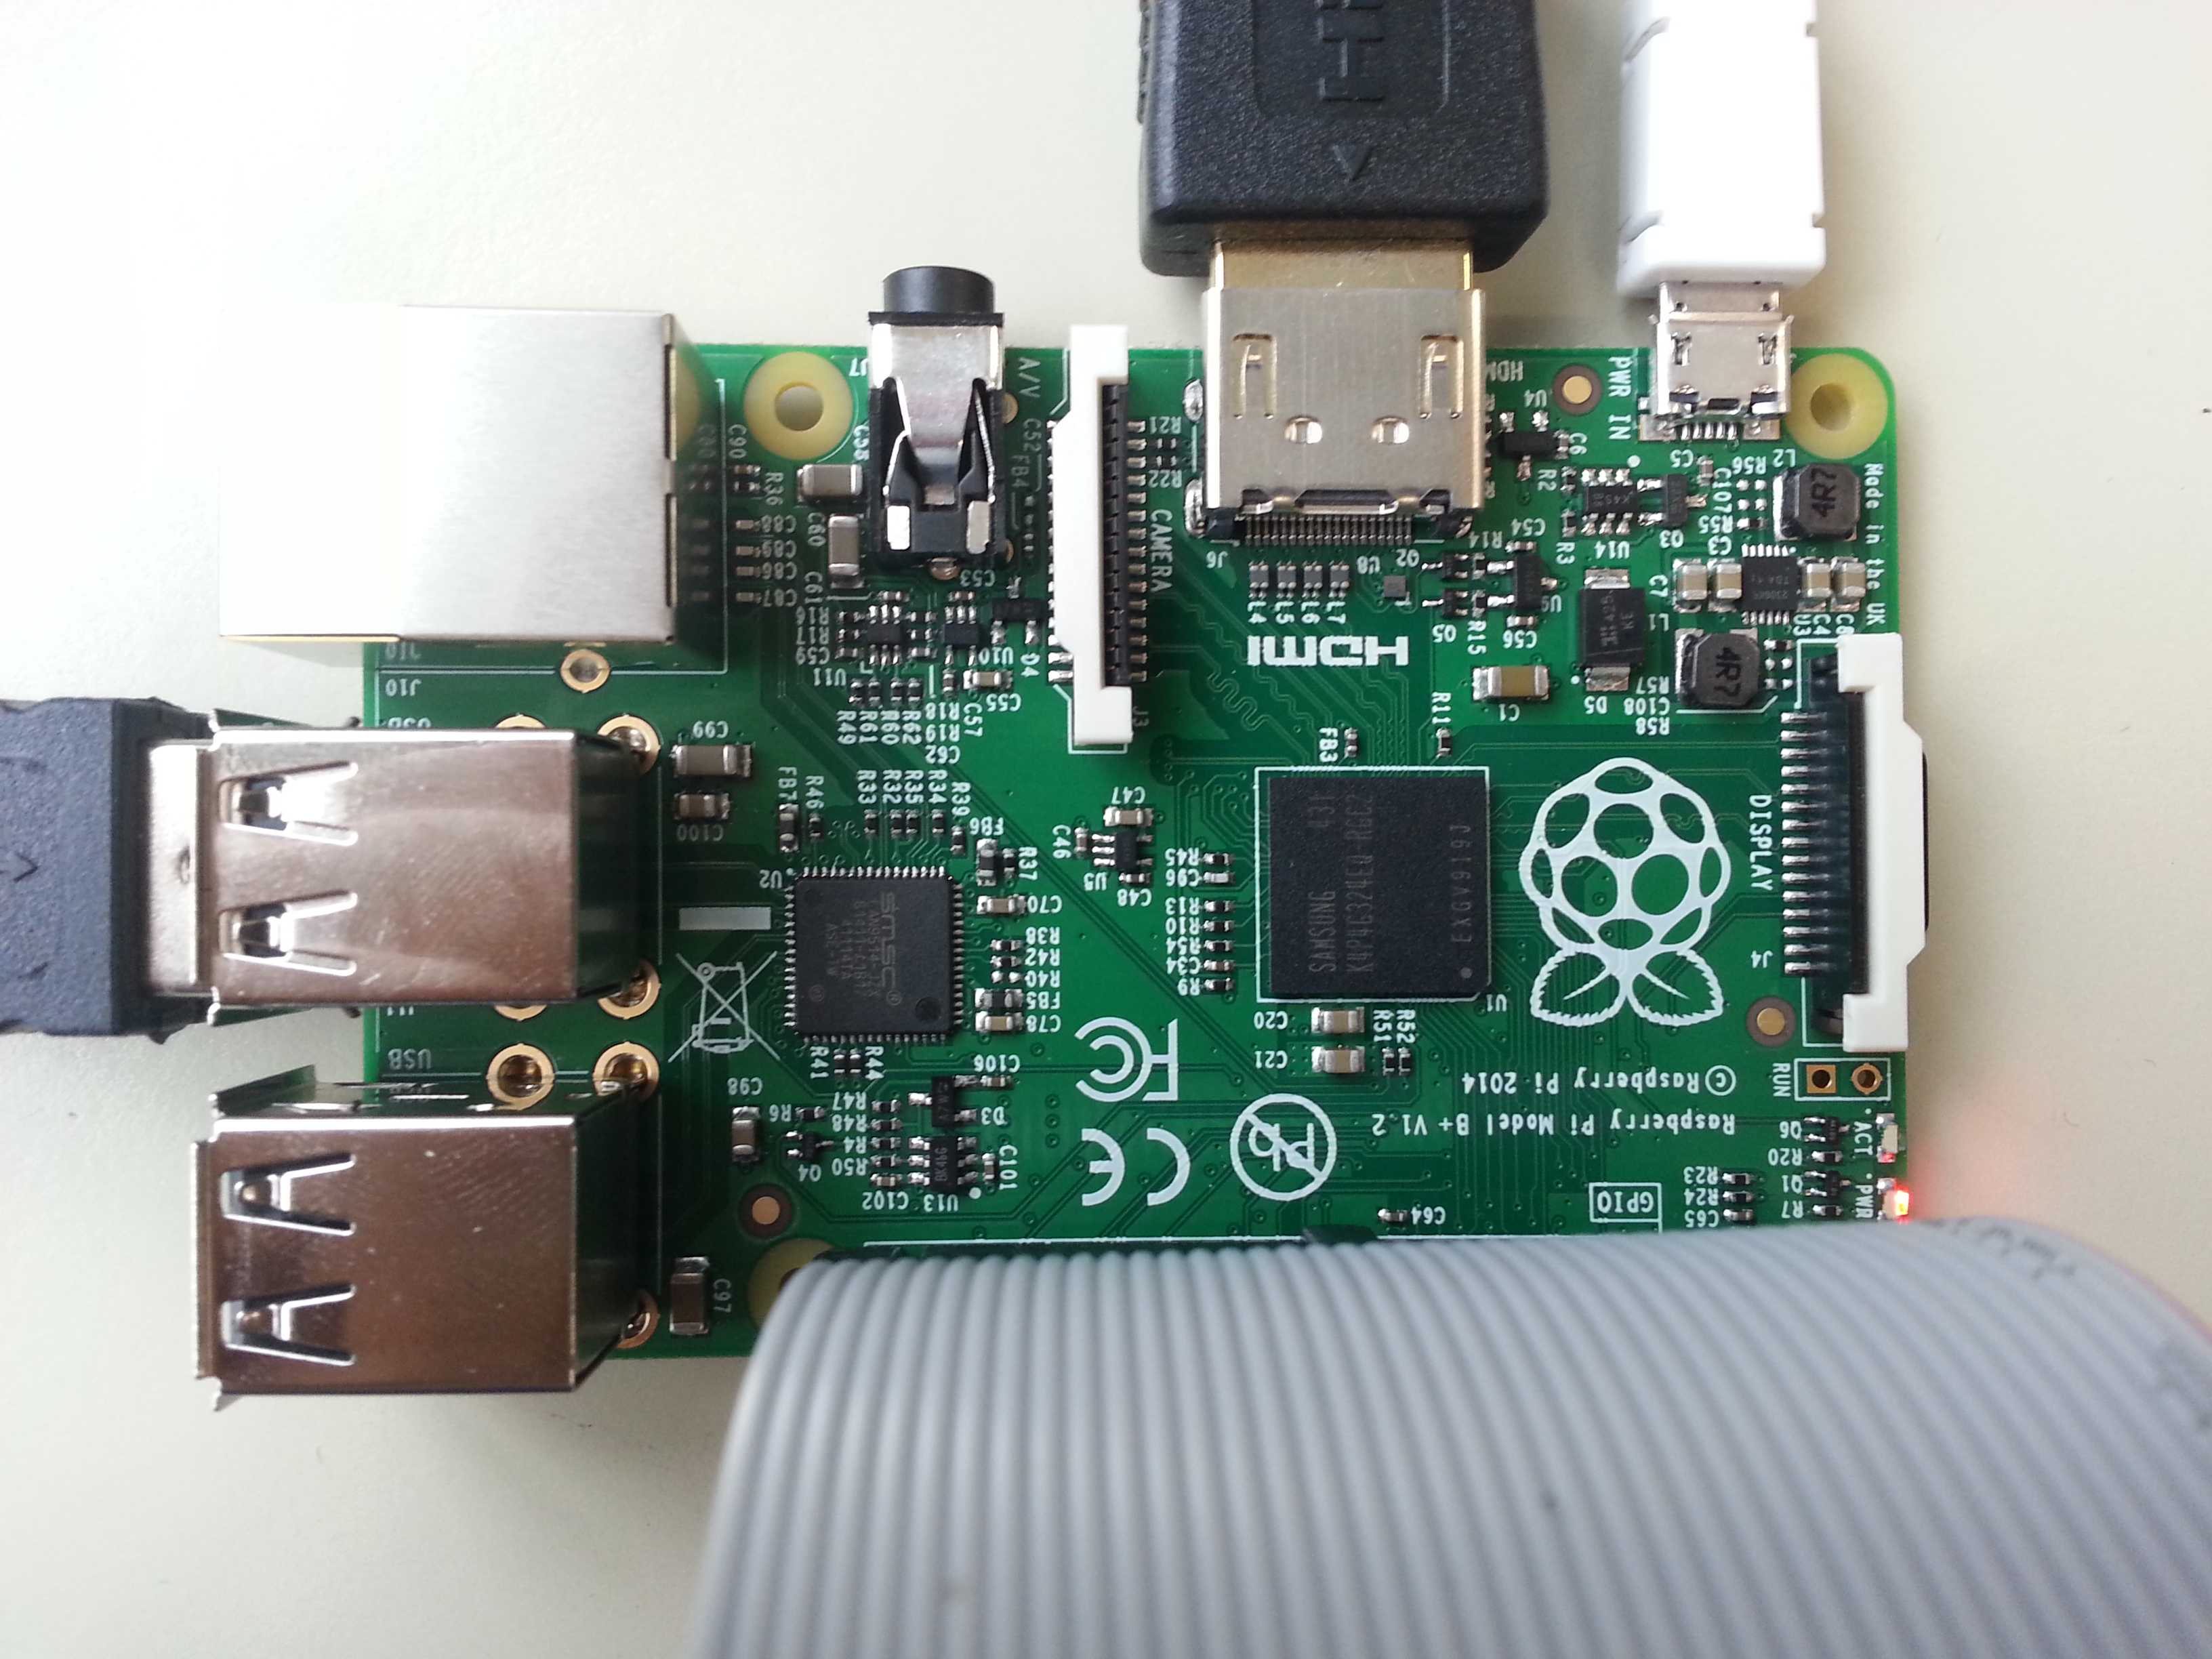
\includegraphics[width=\textwidth]{Test_unitaire/Rpi/img5.jpg}
\captionof{figure}{Notre Raspberry Pi B+}

~\\
\parindent=15pt

Pour s'assurer que notre Raspberry Pi répond aux spécifications fonctionnelles et qu'il fonctionne correctement en toutes circonstances pour notre projet, nous y avons réalisé des tests unitaires.

Après avoir enfin installé le système d'exploitation Raspbian\footnote{La documentation lié à Raspbian est situé en annexe à la page \pageref{annexe:raspbian}} sur notre Raspberry Pi B+, nous avons tenté de tester les ports GPIO. Pour cela, dans un premier temps, nous avons allumé des LED grâce à un script python à travers différents ports GPIO. Sur la figure \ref{figure:led}, on peut observer que nous avons allumé une LED grâce au port 22.
~\\

Dans notre projet le Raspberry Pi sera placé entre le radio-goniomètre à effet Doppler et l'utilisateur. Il aura deux taches, corréler les données entre tous les dispositifs pour obtenir la position du drone et afficher le résultat à l'utilisateur. Pour cela il doit récupérer la direction qui est donné par le Montréal 3v2. Cette position est donnée à travers des LED (voir figure \ref{figure:ledMontreal}). Nous allons donc placer le Raspberry Pi au niveau des LED pour obtenir les informations délivré par le Montréal 3v2. % TODO : A FINIR

\begin{figure}[!h]
  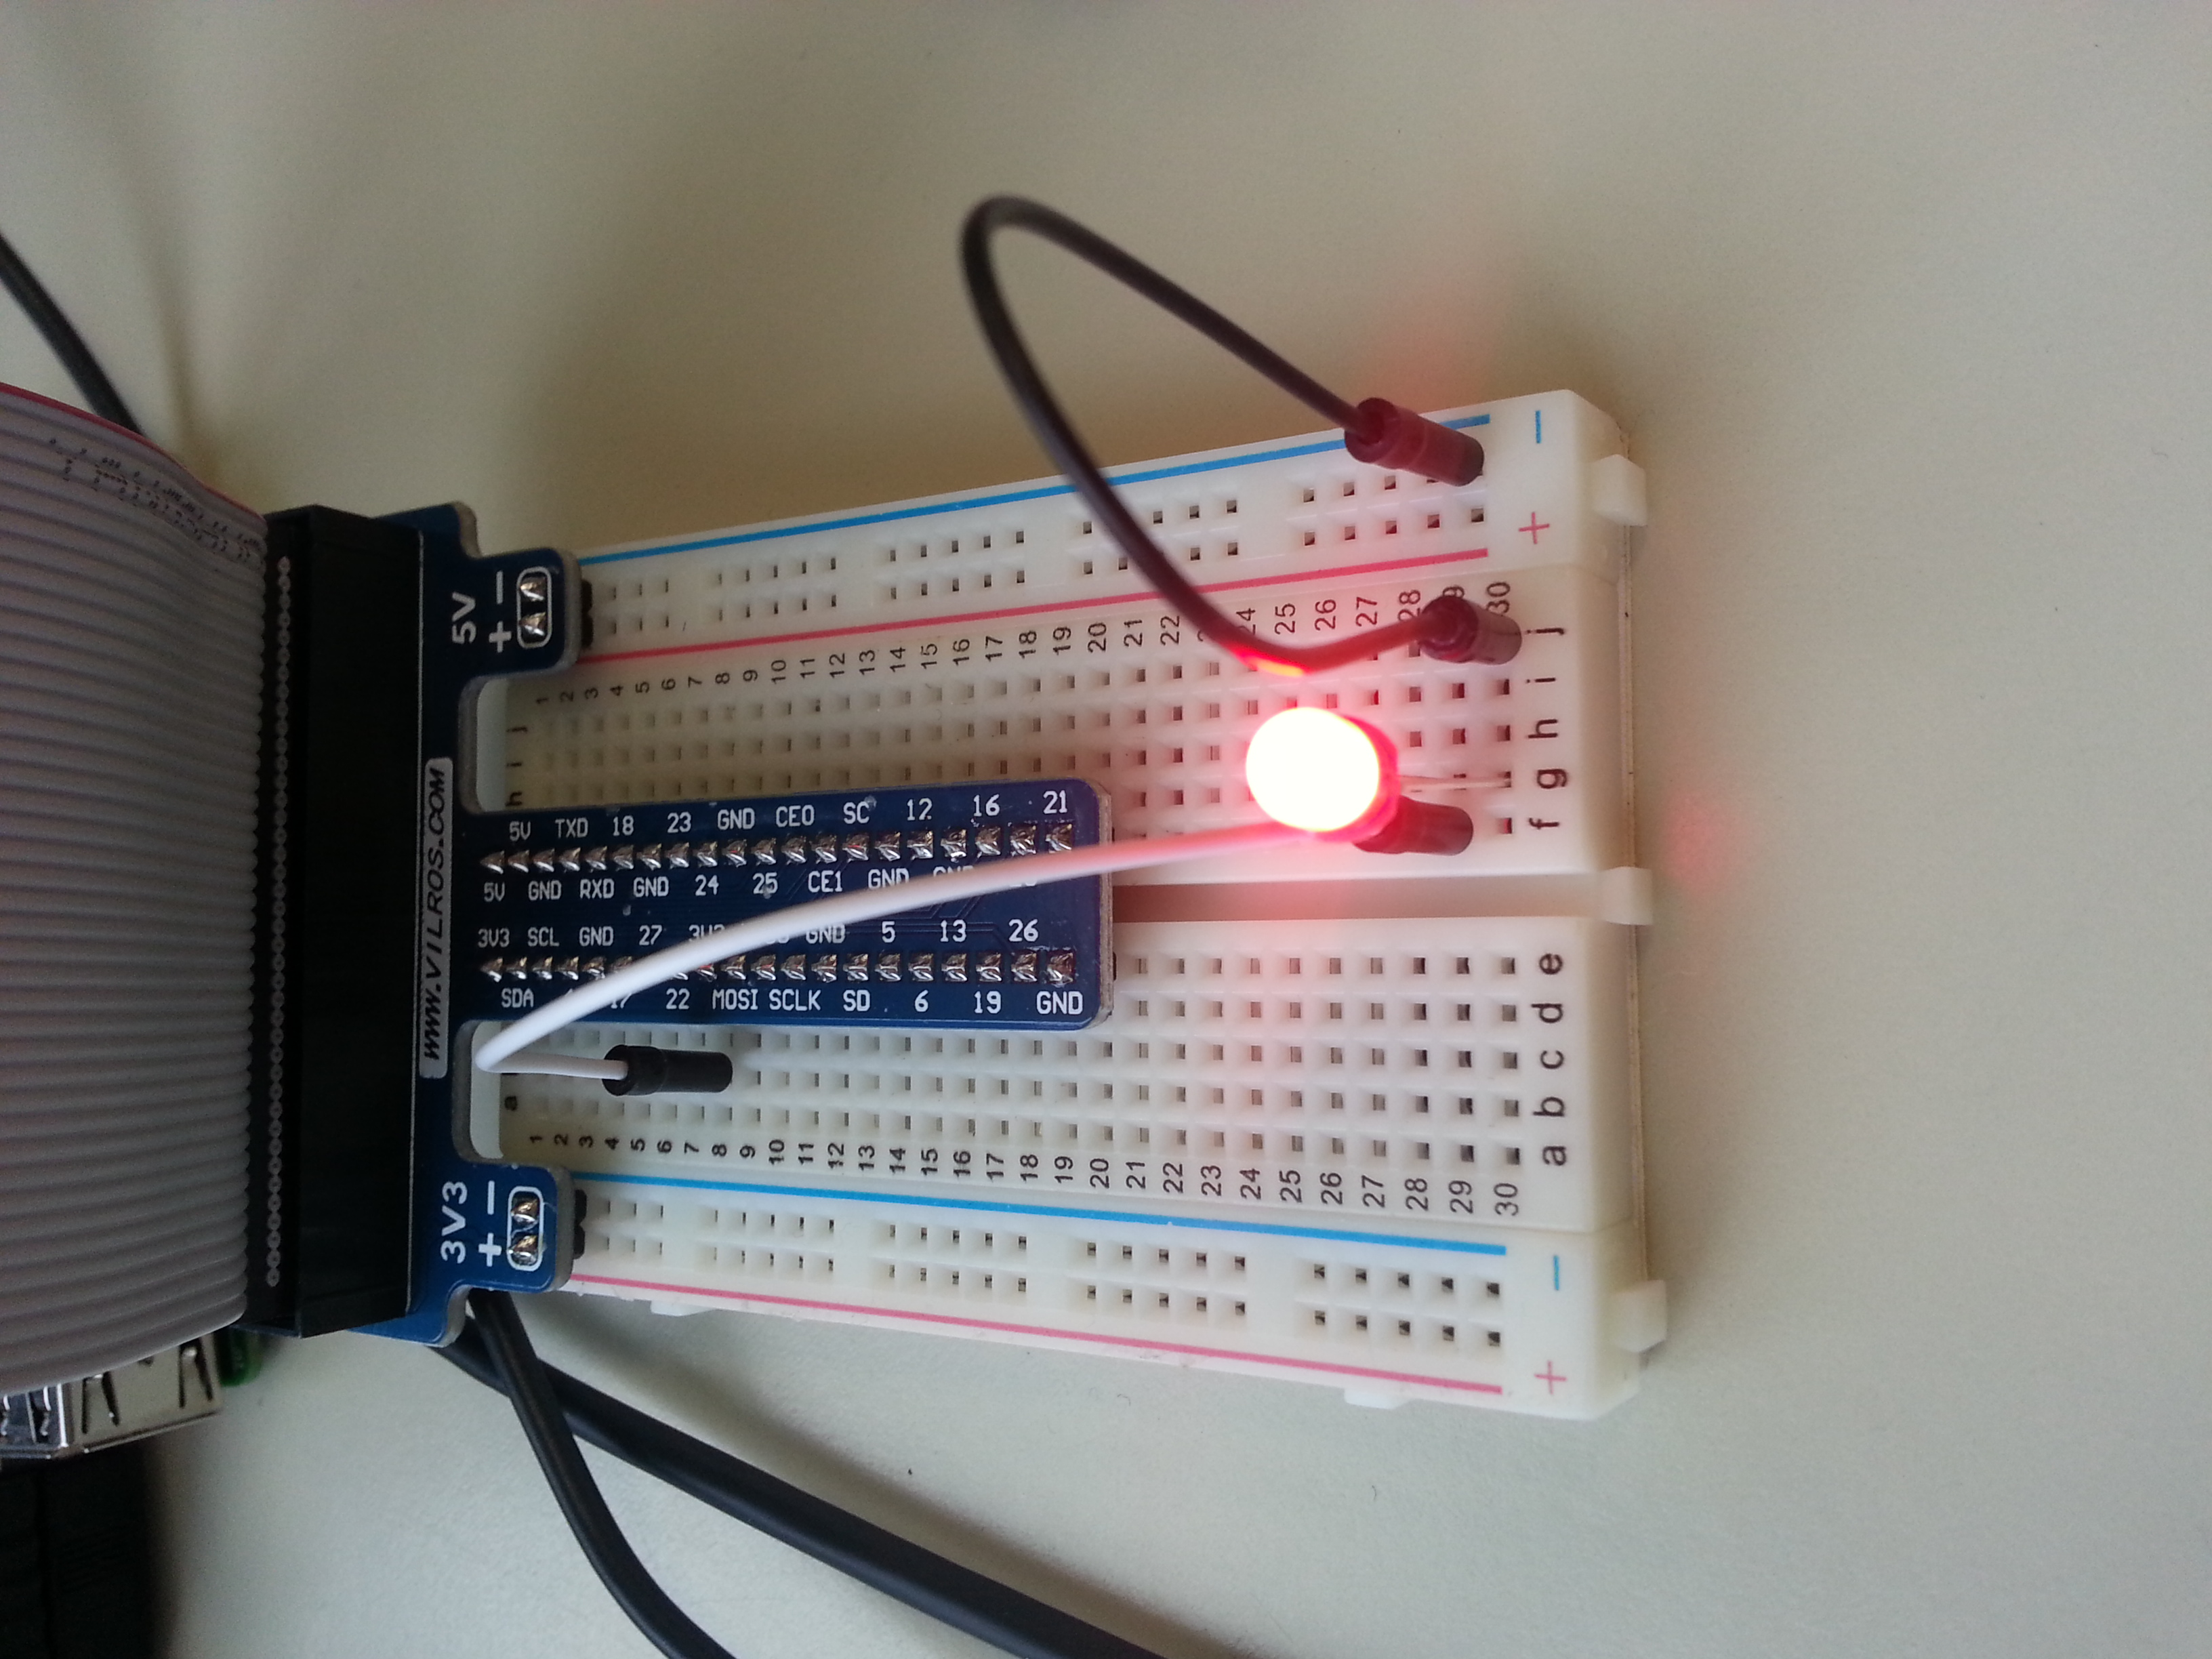
\includegraphics[width=\textwidth]{Test_unitaire/Rpi/img3.jpg}
  \caption{Allumage d'une LED par Raspberry Pi}
  \label{figure:led}
\end{figure}

\begin{figure}[!h]
  \centering
  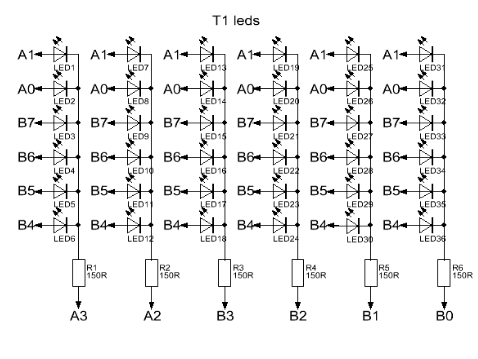
\includegraphics[width=0.8\textwidth]{Test_unitaire/Rpi/led.png}
  \caption{Méthode de connexion des leds dans le Montréal}  
  \label{figure:ledMontreal}
\end{figure}
\begin{figure}[!h]
  \centering
  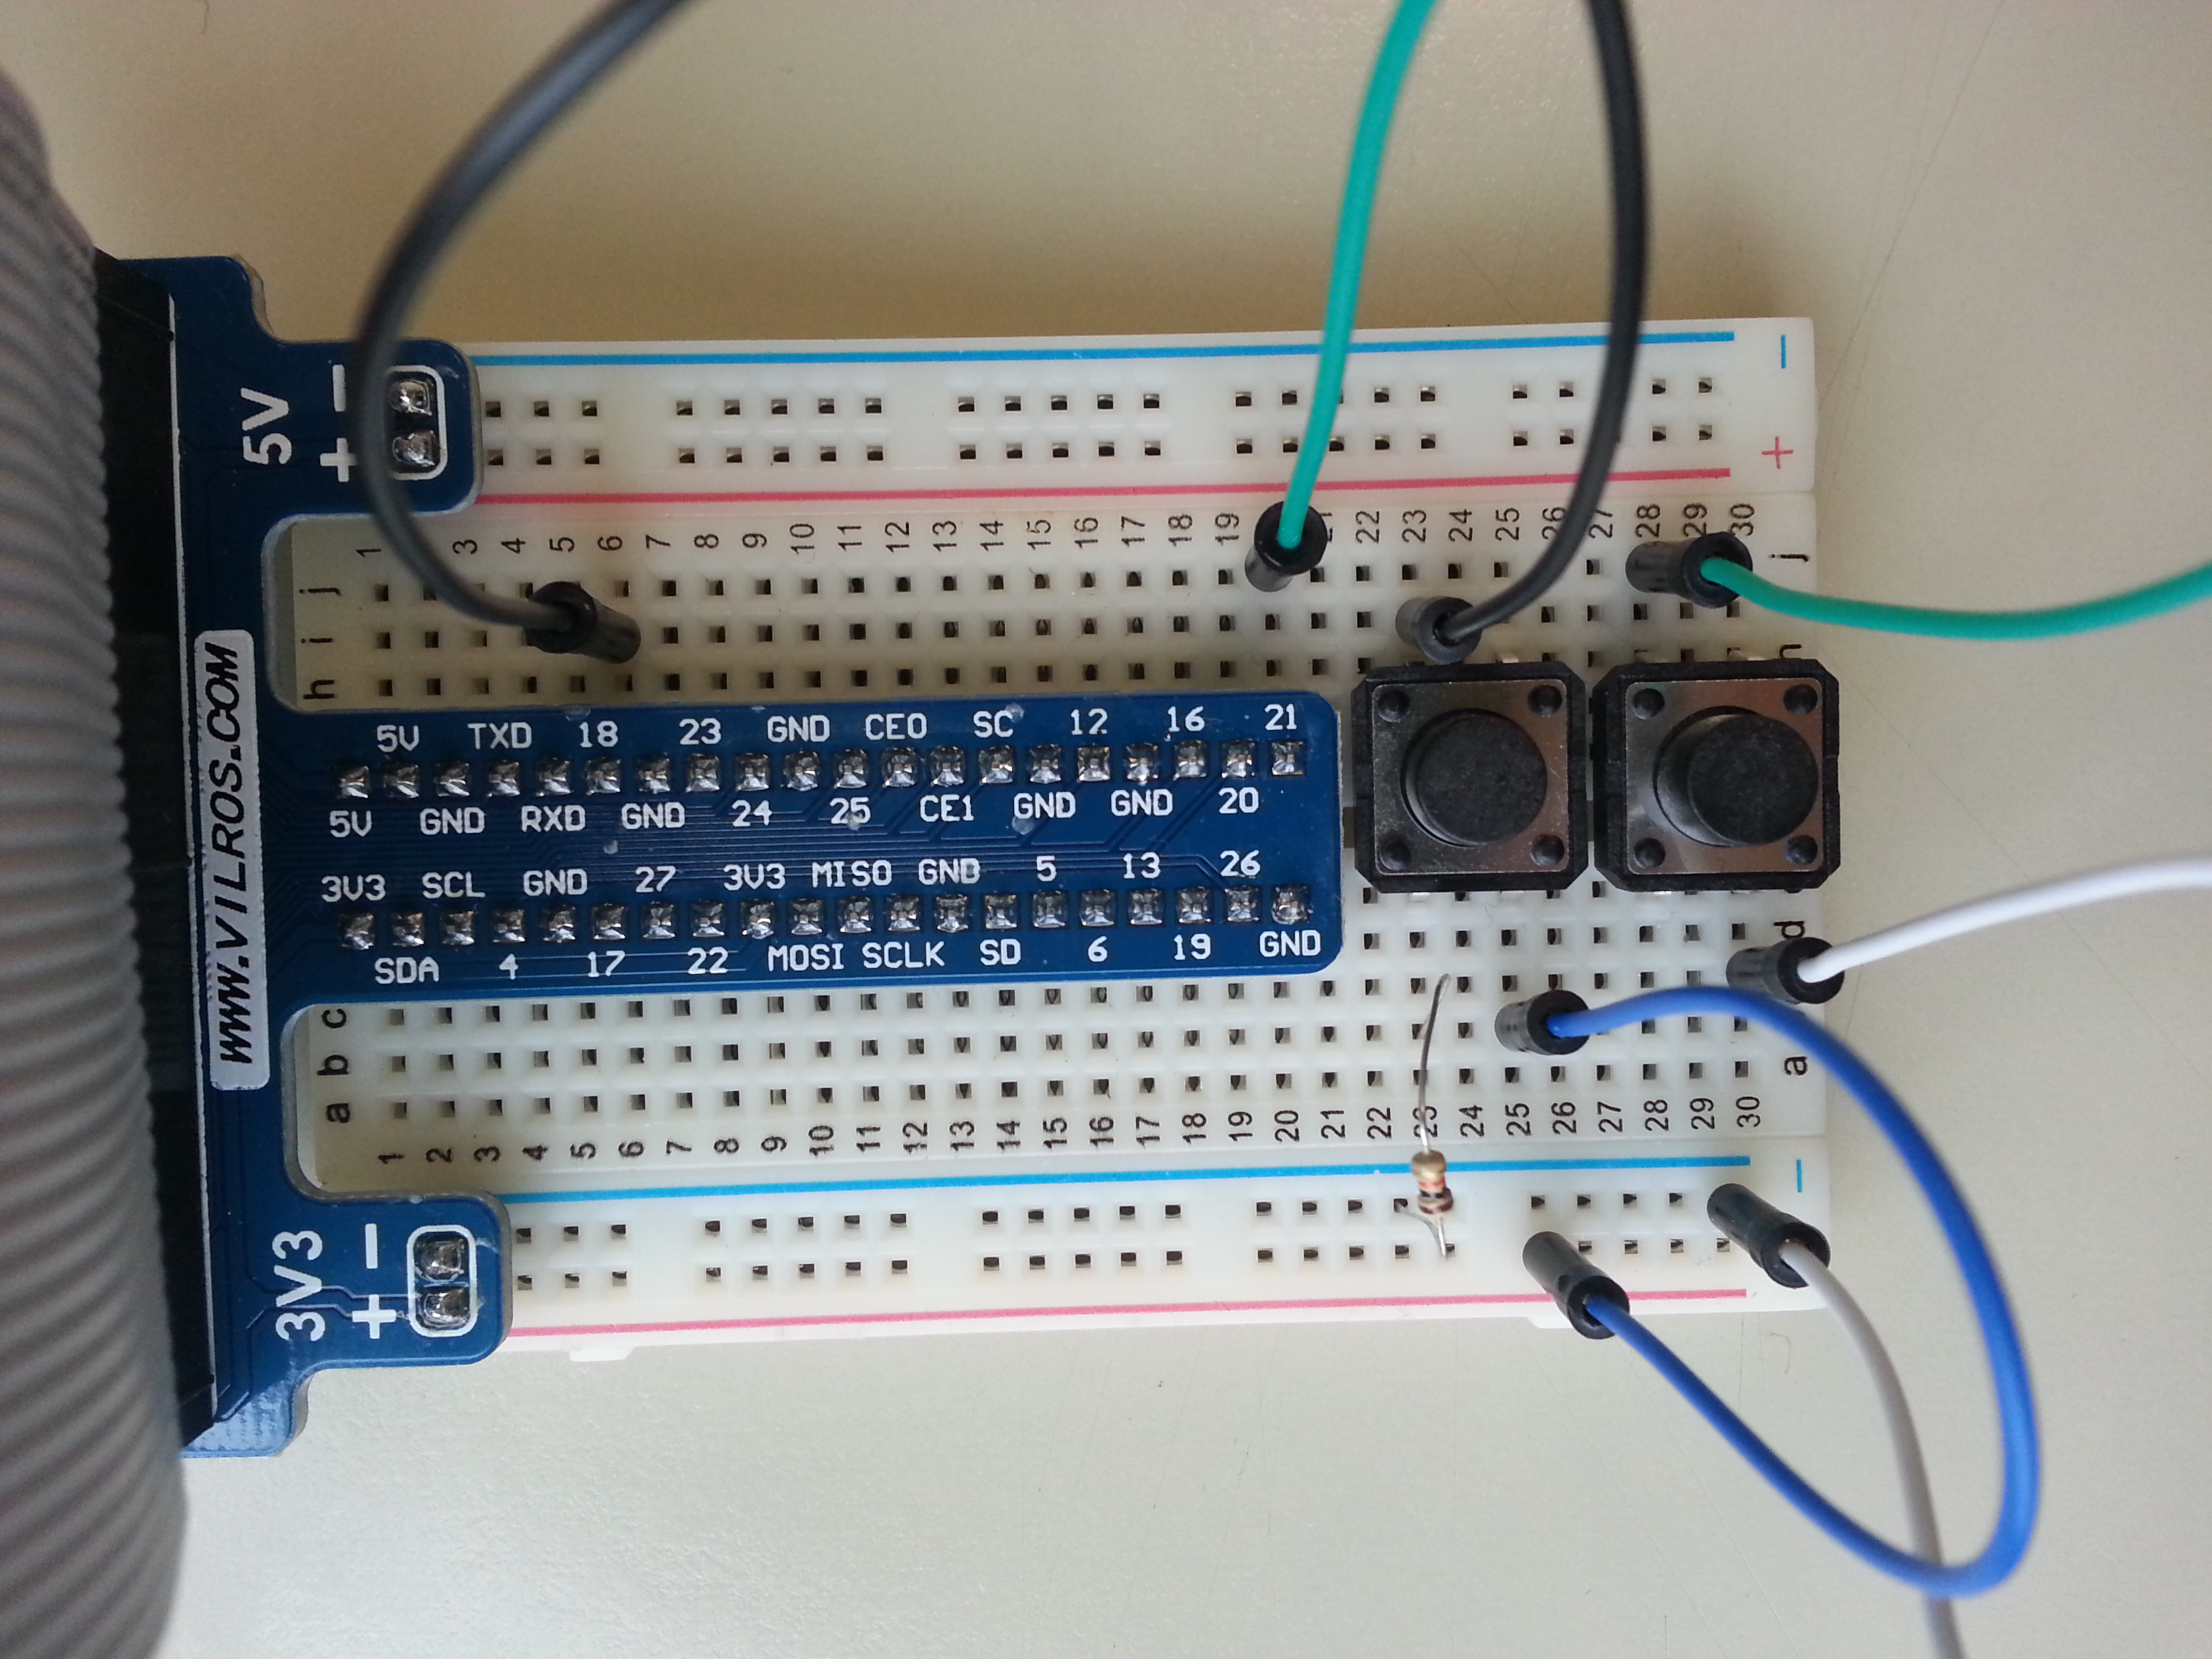
\includegraphics[width=\textwidth]{Test_unitaire/Rpi/img4.jpg}  
  \caption{Système modélisant une LED}
  \label{figure:test}
\end{figure}

La sortie du Montréal 3v2 est décrite à la figure \ref{figure:ledMontreal}. On constate que le pic qui permet l'affichage à 12 sortie qui lui permet de gérer 24 LED. Pour connaître quelle LED est allumé, il faut savoir laquelle des entré A1,A0,B7,B6,B5,B4 à un front montant et laquelle des entrées B0,B1,B2,B3,A3,A2 à un front descendant.

Pour modéliser une LED en entré du Raspberry Pi, nous avons positionné 2 boutons poussoirs (voir figure \ref{figure:test}). Le premier permets de réaliser le front montant et le second le front descendant. Ainsi en positionnant ces boutons au bon endroit par rapport au port GPIO du raspberry il est possible de connaître quelle LED on a simuler.

Nous avons réaliser un script python qui lié les entrées du raspberry avec les sortie du pic. Puis nous avons tester en simulant une LED comme décrit précédemment.

On peut constater que l'expérience est un succès car le raspberry pi nous renvoie bien le numéro de la LED que nous voulions tester.




%%%%%%%%%%%%%%%%%%%%%%%%%%%%%%%%%%%%%%%%%%%%%%%%%%%

\section{PIC}
\label{sec:pic}

Dans le schéma du Montréal 3v2 nous avons pu constater qu'il y avait 3 PIC programmés. Nous avons commandé les PIC programmés au près de l'entreprise F1LVT \cite{montreal}.


\begin{figure}[!h]
  \centering
  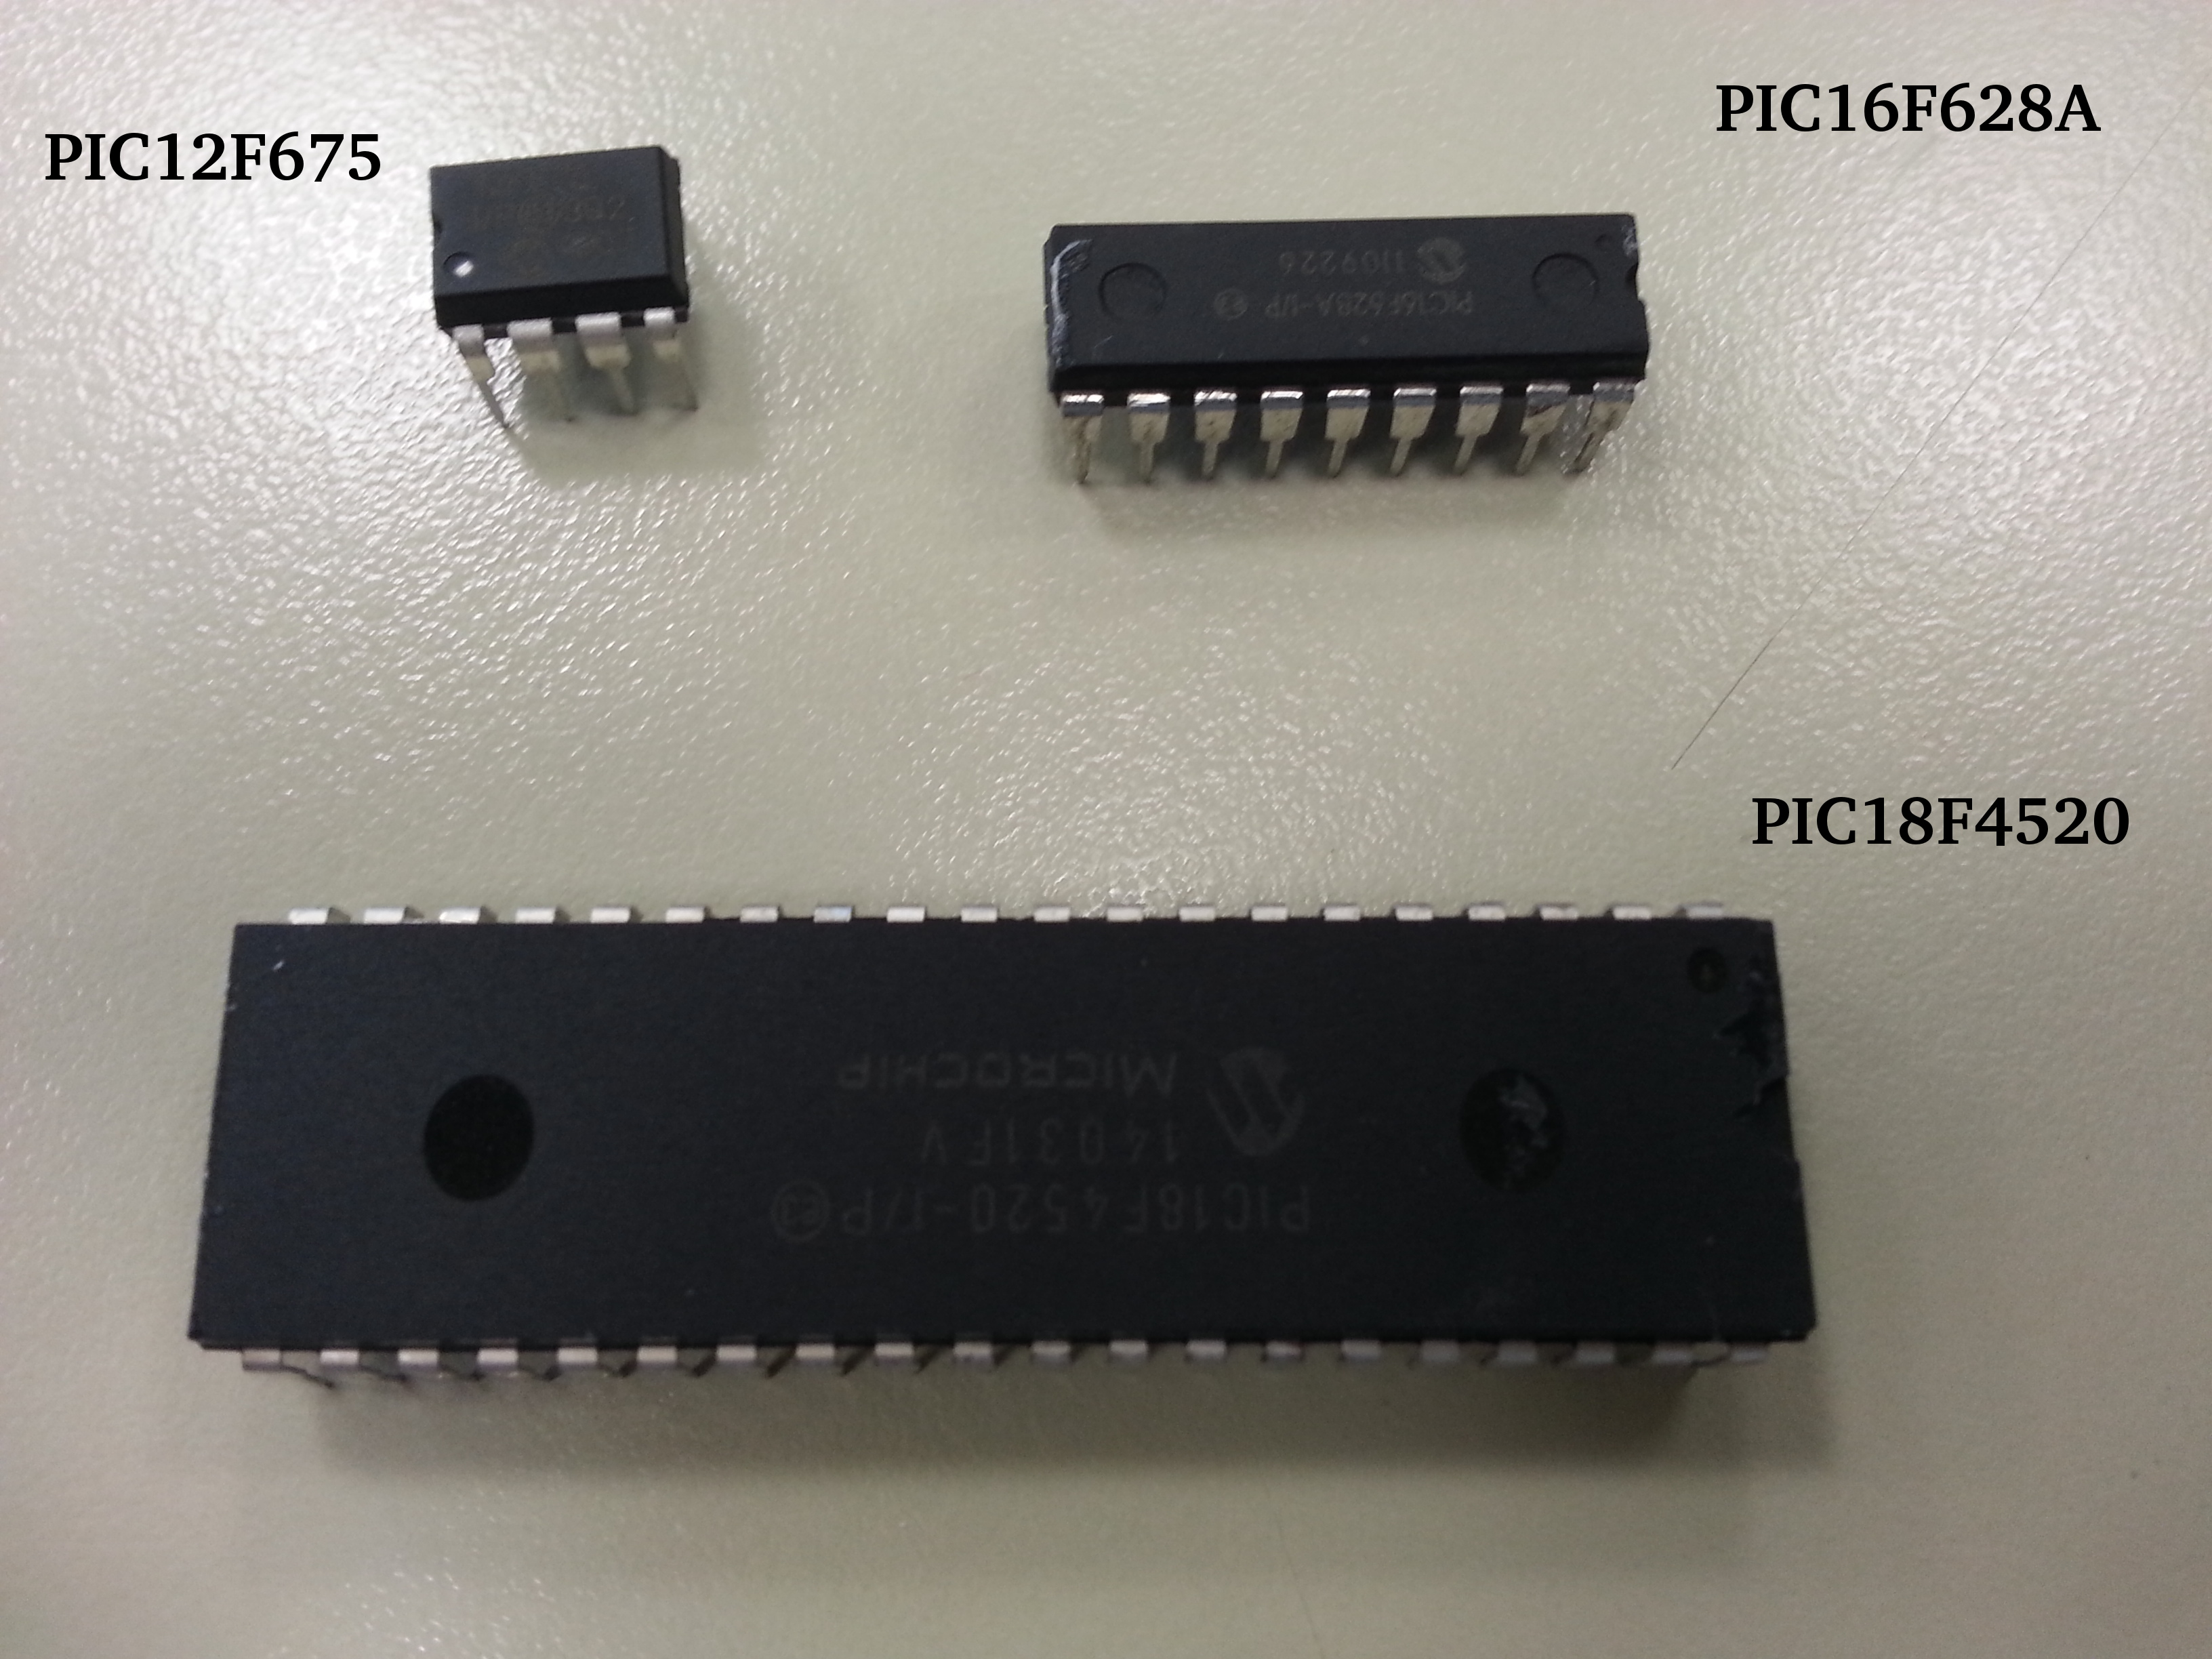
\includegraphics[width=\textwidth]{Test_unitaire/Pic/pic}
  \caption{3 PIC programmés}
  \label{fig:pic}
\end{figure}

Nous avons ensuite imaginé et réalisé des tests unitaires sur chacun des PIC pour vérifier qu'ils ont bien été programmés et qu'aucune erreur n'est apparu sur ce système de décision critique pour le système.

\subsection{PIC16F628A}
\label{sec:picled}

Ce PIC sert à réaliser l'affichage sur les LED. Pour tester ce PIC, nous avons réaliser le montage de la figure \ref{fig:picled}. On peut voir à la figure \ref{fig:schemapic} le schéma de montage du PIC sur le Montréal 3v2.

\begin{figure}[!h]
  \centering
  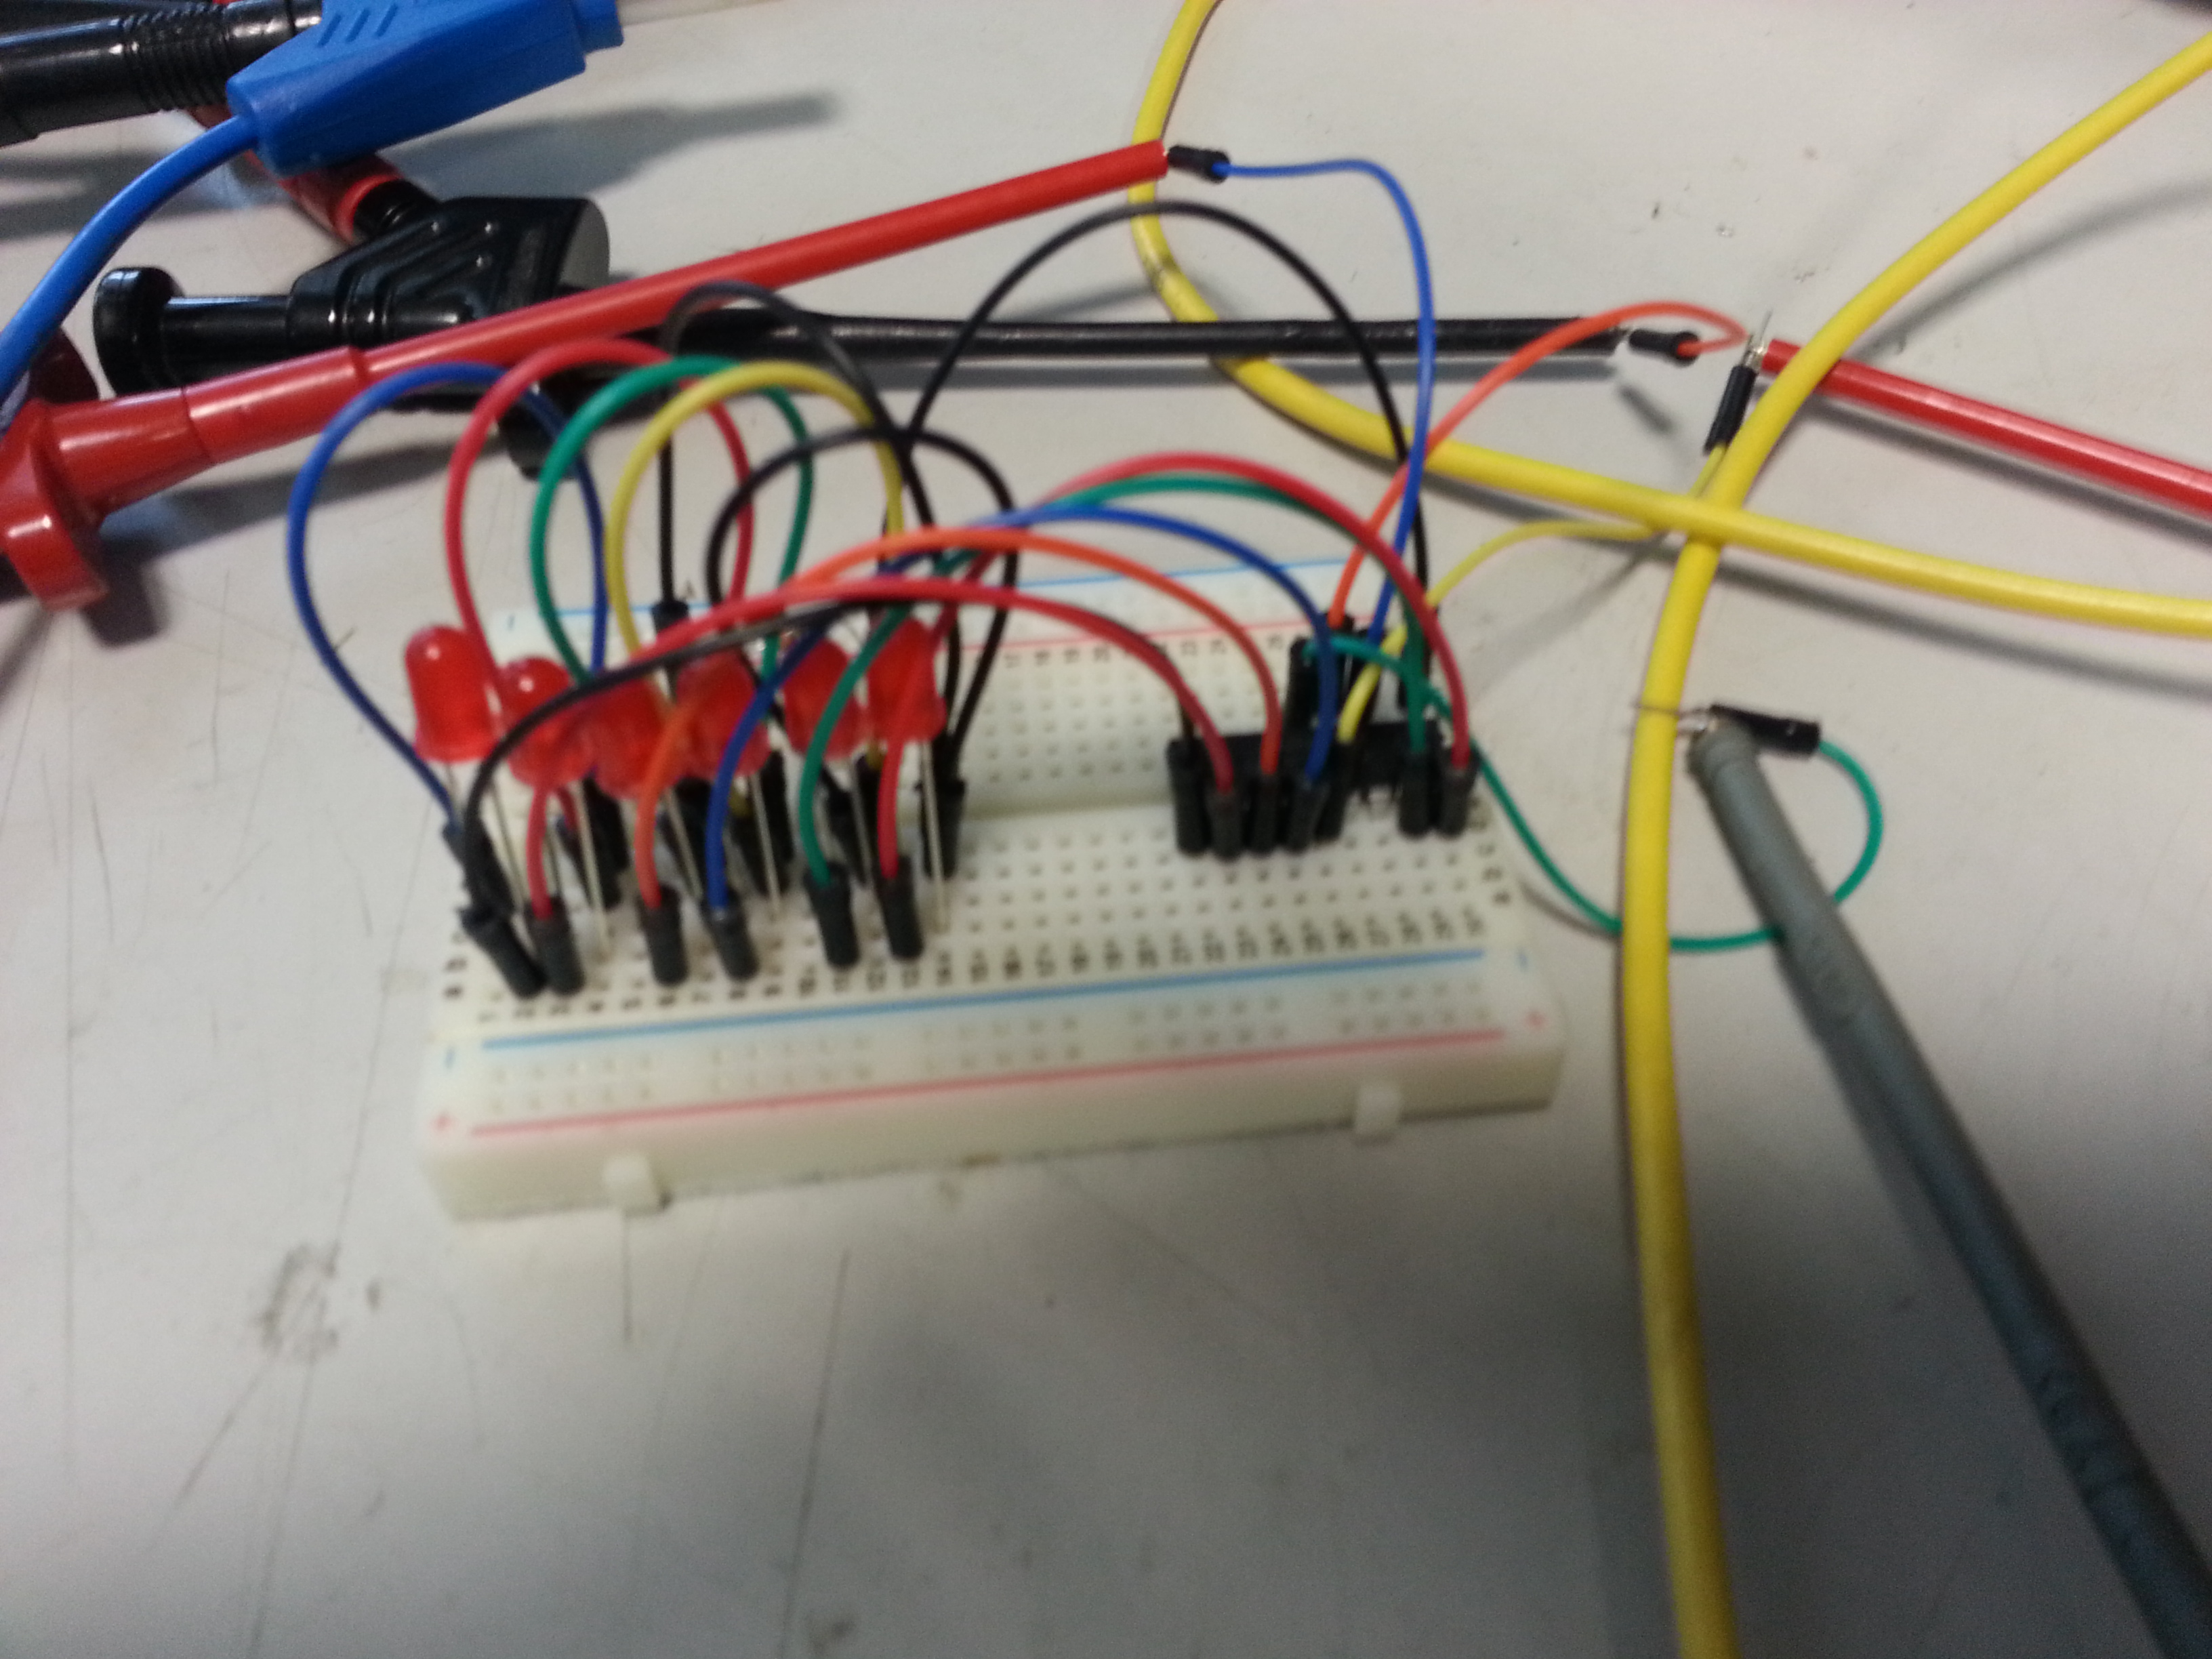
\includegraphics[width=\textwidth]{Test_unitaire/Pic/picled}
  \caption{Schéma electrique du test unitaire}
  \label{fig:picled}
\end{figure}


Pour tester ce composant, nous avons donc choisi de monter une partie des LED situés en sorti, de configurer le \og clock\fg{} sur un signal carré de fréquence 1 MHz, et de faire varier la fréquence de l'entrée \og data\fg{}.

Malheureusement nous n'avons pas pu observer de LED s'allumer pendant notre expérience.

\begin{figure}[!h]
  \centering
  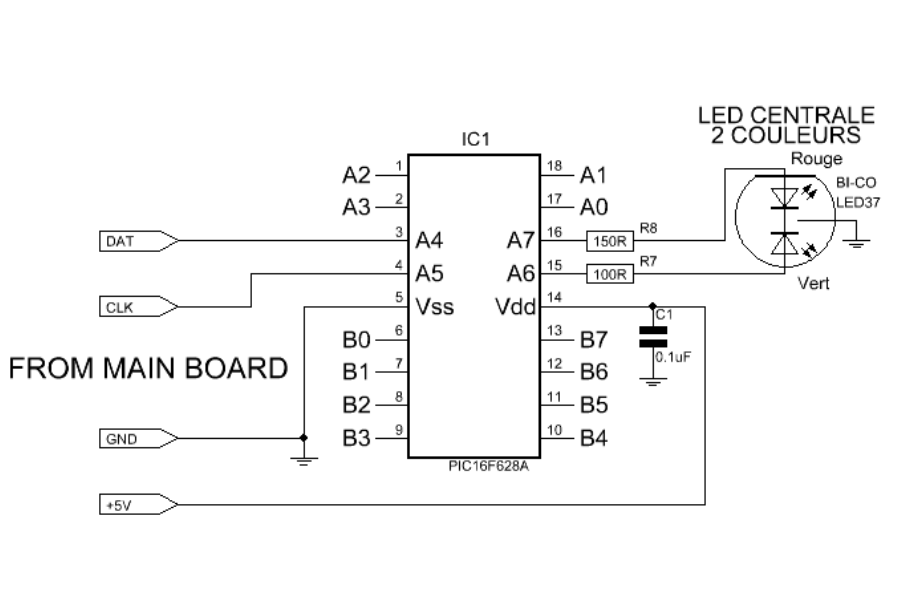
\includegraphics[width=\textwidth]{Test_unitaire/Pic/schemapic}
  \caption{Schéma de montage du pic sur le Montréal 3v2}
  \label{fig:schemapic}
\end{figure}

\subsection{PIC12F675}
\label{sec:picclock}

\subsection{PIC18F4520}
\label{sec:piccontrol}



%%% Local Variables: 
%%% mode: latex
%%% TeX-master: "../rapport"
%%% End: 
